% !TeX spellcheck = en_GB
\section{Surface snowfall accumulation}%\label{sec:sfc_acc}
The surface accumulation is a good point to start to see, if the retrieved snowfall amounts at the surface catch the boundary condition as of the double fence. Precipitation amount at the surface are shown in \Cref{fig:sfc_acc}. The figures are representing the observed surface precipitation accumulation in \SI{}{\mm} over \SI{48}{\hour}. Accumulation, measured by the double fence are presented as purple hexagons. Minutely retrieved surface snowfall amount in dash-dotted orange. The ten \SI{48}{\hour} forecast ensemble members are lines in black and grey, the deterministic and its perturbed ensemble members, respectively. The blue dashed line shows the ensemble mean of all ten members. Since the deterministic and the first ensemble member are having values every hour and the other perturbed members only every three hours, shows the ensemble mean the precipitation amount at 0\SI{0}{\hour}, \SI{3}{\hour}, $\ldots$, \SI{21}{\hour}, \SI{24}{\hour}, $\ldots$, \SI{48}{\hour} forecast time. 
Underneath is the associated \SI{10}{\minute} average wind of the last hour from the \SI{10}{\metre} weather mast at Haukeliseter, to see if surface accumulation observations are influenced by wind. 
%%% image surface accumulation %%%%%%%%%%%%%%%%%%%%%%%%%%%%%%%%%%%%%
% !TeX spellcheck = en_GB
%\begin{landscape}
\begin{figure}[t!]
	\centering
	% 21/12
	\begin{subfigure}[t]{0.49\textwidth}		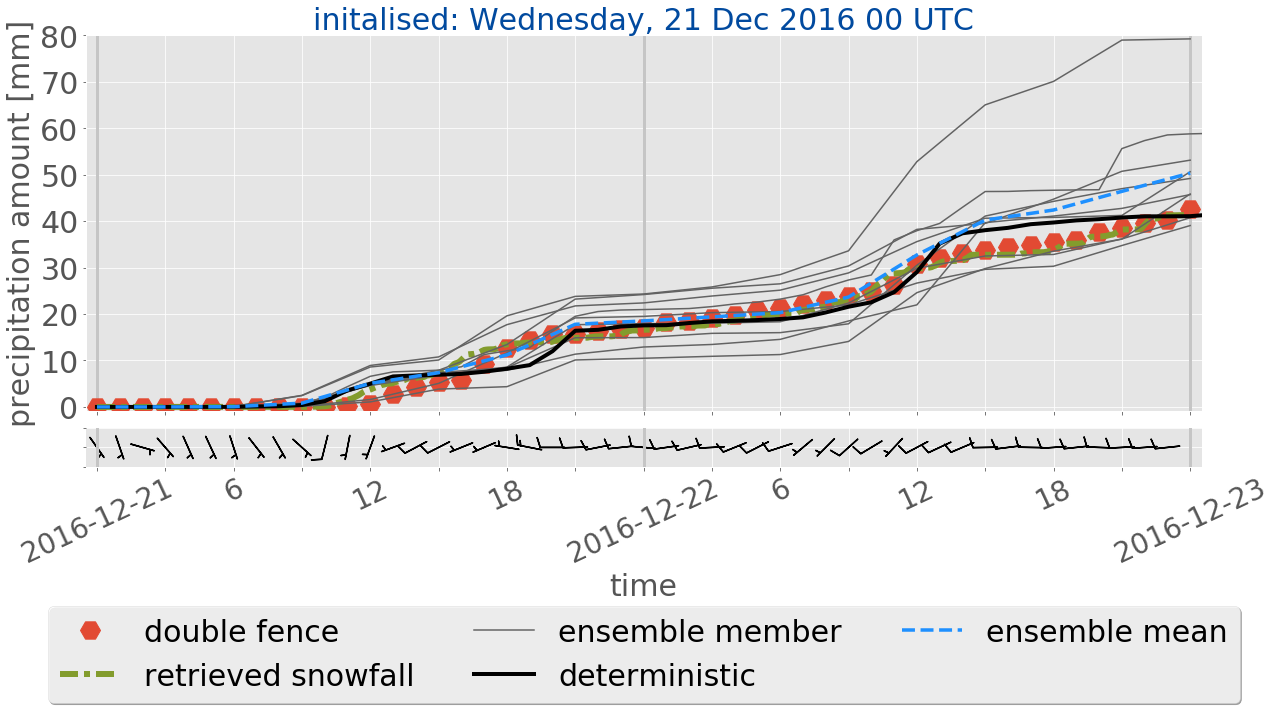
\includegraphics[trim={3.cm 2.6cm 2.cm 1.9cm},clip,width=\textwidth]{./fig_sfc_acc/acc_wind_20161221_00}
		\caption{}\label{fig:sfc_acc21}
	\end{subfigure}
	% 22/12
	\begin{subfigure}[t]{0.49\textwidth}		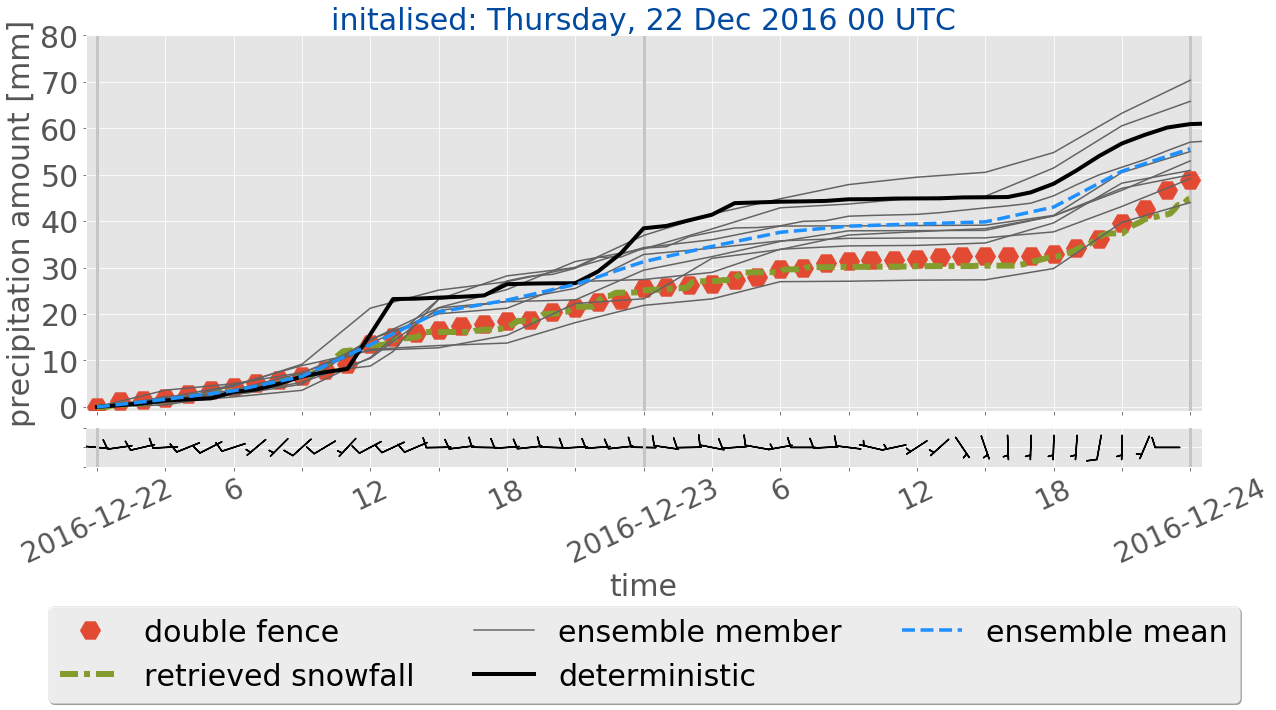
\includegraphics[trim={3.cm 2.6cm 2.cm 1.9cm},clip,width=\textwidth]{./fig_sfc_acc/acc_wind_20161222_00}
		\caption{}\label{fig:sfc_acc22}
	\end{subfigure}
	%	\end{figure}
	%   \begin{figure}\ContinuedFloat
	% 23/12
	\begin{subfigure}[t]{0.49\textwidth}	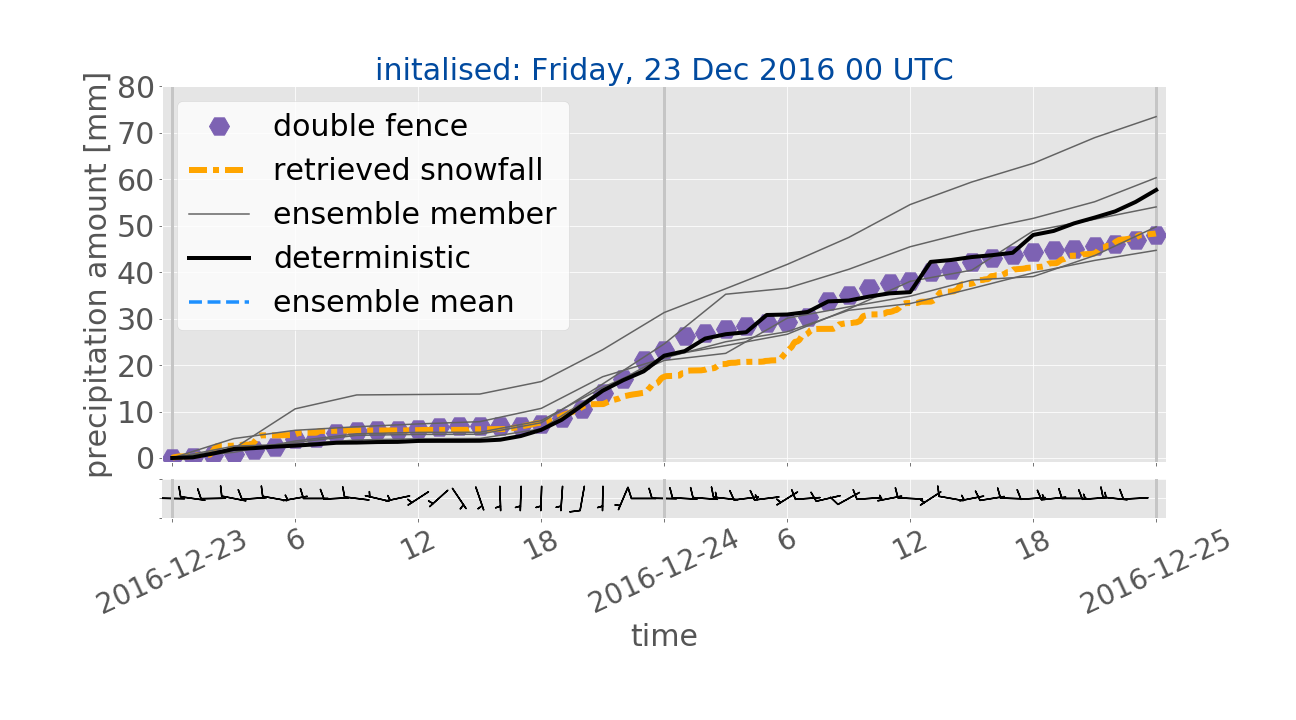
\includegraphics[trim={3.cm 2.6cm 2.cm 1.9cm},clip,width=\textwidth]{./fig_sfc_acc/acc_wind_20161223_00}
		\caption{}\label{fig:sfc_acc23}
	\end{subfigure}
	% 24/12
	\begin{subfigure}[t]{0.49\textwidth}			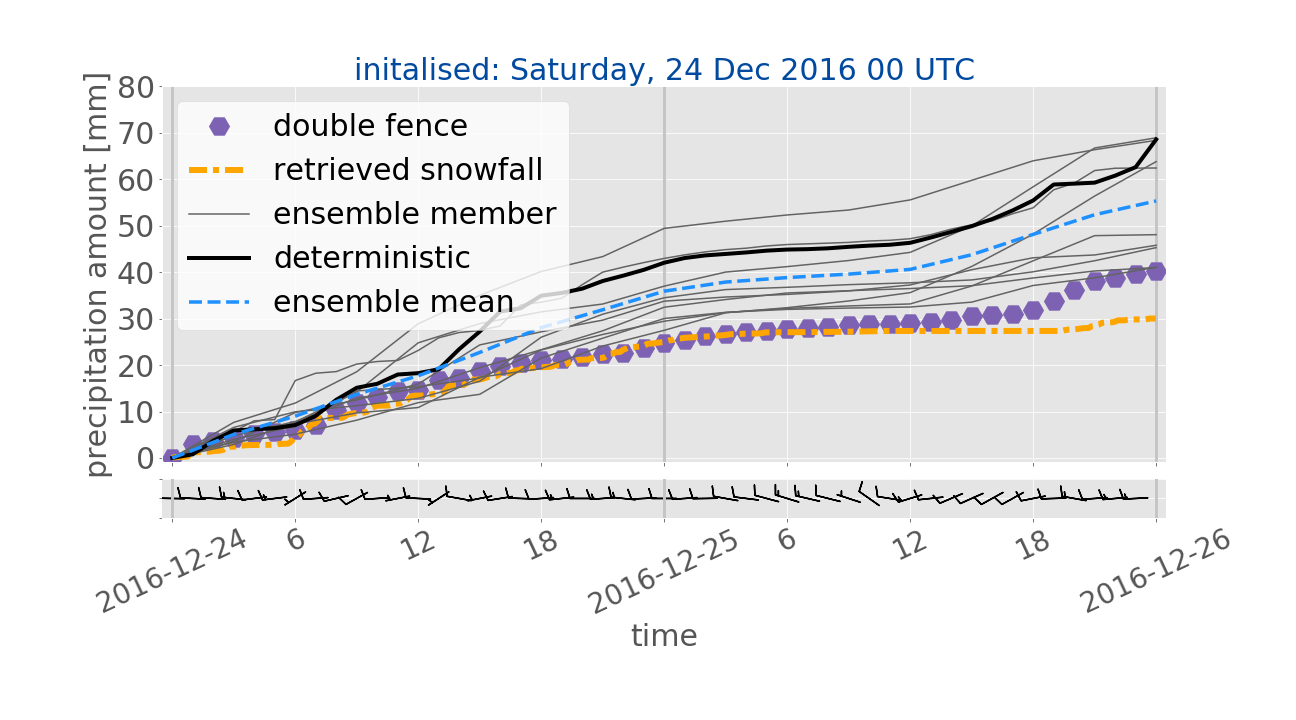
\includegraphics[trim={3.cm 2.6cm 2.cm 1.9cm},clip,width=\textwidth]{./fig_sfc_acc/acc_wind_20161224_00}
		\caption{}\label{fig:sfc_acc24}
	\end{subfigure}
	% 25/12
	\begin{subfigure}[t]{0.49\textwidth}
		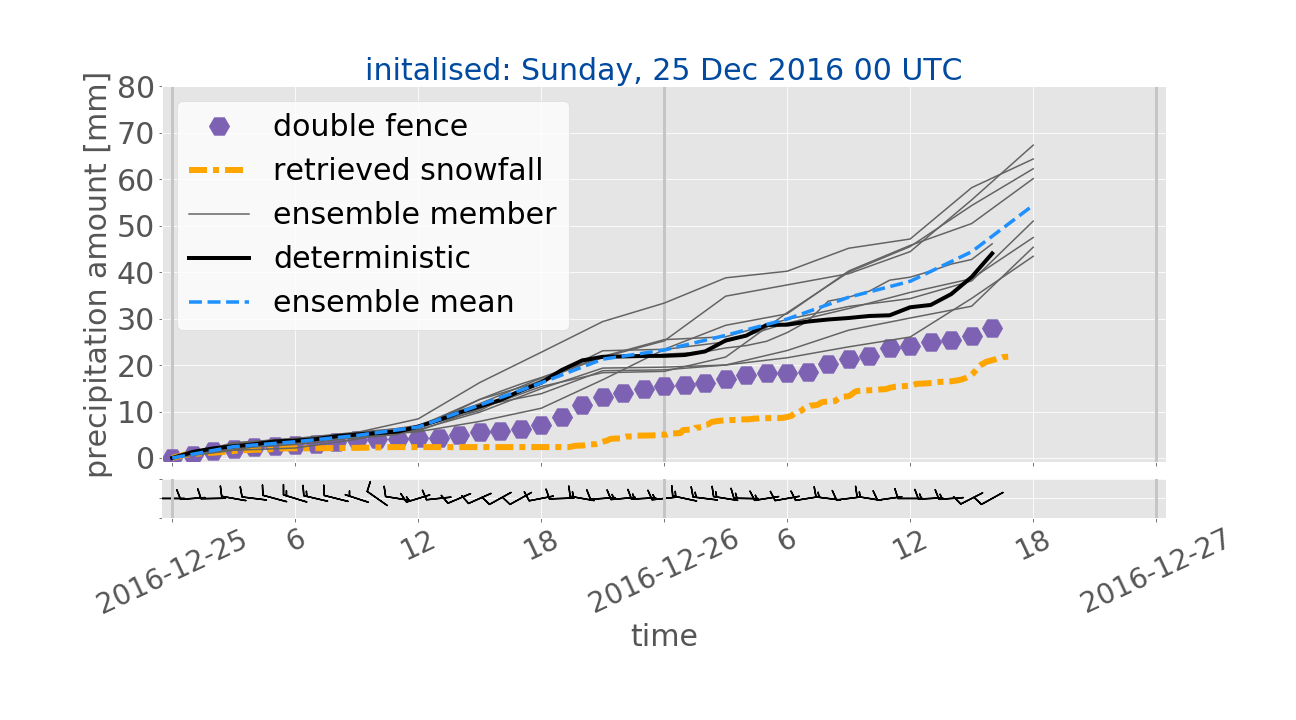
\includegraphics[trim={3.cm 2.6cm 2.cm 1.9cm},clip,width=\textwidth]{./fig_sfc_acc/acc_wind_20161225_00}
		\caption{}\label{fig:sfc_acc25}
	\end{subfigure}
	% 26/12
	\begin{subfigure}[t]{0.49\textwidth}	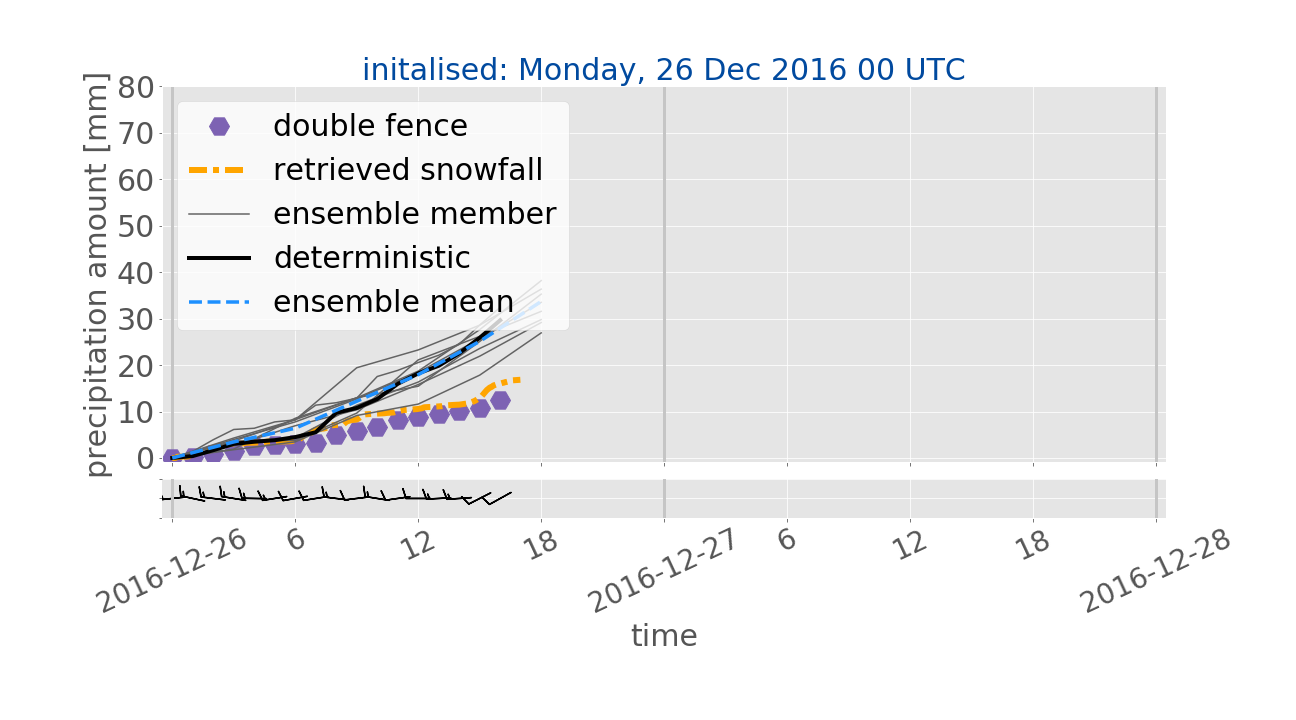
\includegraphics[trim={3.cm 2.6cm 2.cm 1.9cm},clip,width=\textwidth]{./fig_sfc_acc/acc_wind_20161226_00}
		\caption{}\label{fig:sfc_acc26}
	\end{subfigure}
	\caption{Surface snowfall accumulation. Representing the values from the double fence in purple, hexagons; optimal estimation retrieval output at snow layer height \SI{800}{\metre} in dash-dotted orange; and ensemble member deterministic forecast, initialised at 0\SI{00}{\UTC} in black and its nine perturbed ensemble members in grey. The ensemble mean of all ten members is shown in blue dashed.  Underneath are the associated last \SI{10}{\minute} average wind from the weather mast at \SI{10}{\metre} height. }\label{fig:sfc_acc}
\end{figure}



%%%%%%%%%%%%%%%%%%%%%%%%%%%%%%%%%%%%%%%%%%%%%%%%%%%%%%%%%%%%%%%%%%%%%%%%%%
\noindent
In general show the \SI{48}{\hour} surface accumulation in \Cref{fig:sfc_acc21,fig:sfc_acc22,fig:sfc_acc23} a good agreement between the foretasted values and the retrieved snowfall amount when comparing to the double fence. \SI{24}{\dec} and \SI{25}{\dec} show a disagreement between the surface observations and the model forecast. During this days is the precipitation amount predicted by MEPS for all ten ensemble members higher than for the measured accumulation. The possible reason for the overestimation at the ground is later discussed in \Cref{sec:2412:surface} and \ref{sec:2512:surface}. \\
Retrieved accumulation almost always reached the boundary condition of the double fence observations. The only well pronounced mismatch is seen on \SI{25}{\dec}, where it measures much less than the double fence gauge.  
\\ \\
The surface accumulation initialised on the \SI{21}{\dec} at 0\SI{0}{\UTC} has one ensemble member overestimating the precipitation amount after \SI{33}{\hour} forecast time. Otherwise, agree all three systems well with each other and the perturbed ensemble members are equally spread around the deterministic forecast.
\\
On \SI{22}{\dec} (\Cref{fig:sfc_acc22}) fit the ensemble mean relatively well to the observed surface accumulation, were the double fence estimates the least amount. Clearly, the ensemble members in grey are not equally distributed around the deterministic forecast. The deterministic is predicting more surface accumulation with a large jump after \SI{11}{\hour}, always being higher than most of the ensemble members and observations. 
\\
When too few ensemble members were present, like on \SI{23}{\dec}, no ensemble mean is calculated. \Cref{fig:sfc_acc23} shows a good agreement between the double fence observations and the deterministic forecast. Here, for the first time measures the retrieved surface snowfall accumulation less than for the double fence, but the difference is almost negligible and starts to be too little after \SI{20}{\UTC} on \SI{23}{\dec}. This underestimation might be related to the wind change from weaker south to stronger west wind.
\\
\Cref{fig:sfc_acc24} indicates an overestimation of the deterministic surface snowfall prediction already after \SI{16}{\hour} forecast time, when initialised on \SI{24}{\dec}. The deterministic forecast in solid black is much higher and increases faster than the observations. A higher value of approximately \SI{15}{\mm} can be seen when compared to the surface measurements at \SI{16}{\UTC} on \SI{24}{\dec}. This difference remains almost constantly over the forecast time. Furthermore, all ensemble members seem to overestimate the surface accumulation after \SI{24}{\hour} prediction time. Since MEPS performed on the previous days one might assume, that the double fence gauge measurements are influenced by the surface winds. By comparing the \SI{10}{\minute} average wind at \SI{13}{\UTC} it shows an increase of wind speed from \SI{5}{\mPs} to \SI{10}{\mPs}. In \cite{wolff_wmo_2018} it is stated, that the gauge protected by a double fence is influenced by wind but the error is not too big compared to strong wind higher than \SI{20}{\mPs}. Therefore, it is assumed that the measurements from the double fence are correct and MEPS had rather a forecast error, since the retrieved surface snow accumulation would assume the same precipitation amount. The total accumulated precipitation amount provided in MEPS includes liquid and solid precipitation. The ensemble mean shows also an inaccuracy of forecasted precipitation at the surface. One reason for the overestimation of the accumulation on the ground could be that MEPS has expected a large amount of liquid precipitation, which actually did not occur. A discussion, including a whisker-box-plot from the ensemble members is provided in \Cref{sec:2412:surface}.
\\
On the \SI{26}{\dec} the MRR did not work after approximately \SI{17}{\UTC} and therefore only values before \SI{17}{\UTC} are compared. 
The surface precipitation amount on \SI{25}{\dec} shows again a miscalculation from MEPS in \Cref{fig:sfc_acc25}. After \SI{12}{\hour} forecast time the ensemble members overestimate the surface accumulation, which gets more pronounced at \SI{18}{\UTC}. But still, the model forecast members seem to follow the same structure as the double fence, just too high. Compared to the \SI{24}{\dec} where the ensemble members were not spread equally around the deterministic forecast, shows the \SI{25}{\dec} a good distribution since the ensemble mean is almost the same as the deterministic forecast. 
The retrieved snowfall accumulation seems to be too little over the entire period, when it starts to precipitate more around \SI{18}{\UTC} on the \SI{25}{\dec} in \Cref{fig:sfc_acc25}. This might be, because the optimal estimation retrieval does not account for liquid precipitation, which was observed during this time period. While the double fence gauge measures liquid and solid precipitation could the pure neglection of liquid precipitation follow the disagreement between double fence and retrieved surface accumulation, which will be further discussed in \Cref{sec:2512:surface}.
\\
Because of an instrumentation error after \SI{17}{\UTC} on \SI{26}{\dec} is this day not really representable. From the double fence precipitation measurement in \Cref{fig:TPU26} and \ref{fig:TPU27} it is known that precipitation was continuous present until \SI{27}{\dec} \SI{10}{\UTC}. Nevertheless, \Cref{fig:sfc_acc26} shows an overestimation by MEPS after \SI{12}{\hour} prediction. The spread around the deterministic forecast is relatively narrow with a good agreement between ensemble mean and deterministic. 
\\ \noindent
%%%% DISCUSSION of sfc accumulation %%%%%%%%
% \textcolor{red}{DISCUSS! Why is the surface accumulation predicted better for the first days and not too well for the \SIlist{24;25}{\dec}? From Introduction, since excluded: \\
%
\begin{table}[h]
	\begin{center}
		\caption{Surface snowfall accumulation measured by the double fence gauge. Presenting \SI{12}{\hour} accumulation before noon and after noon, as well as the total \SI{24}{\hour} surface accretion. }\label{tab:sfc_acc}
		\begin{tabular}{c|c|c|c}
			\hline \hline
			\textbf{Day} & \multicolumn{3}{c}{\textbf{Accumulation}} \\ 
			& \multicolumn{3}{c}{[\SI{}{\mm}]} \\ \hline
			& \SI{12}{\hour} (\footnotesize{\num{0} to \SI{12}{\UTC}}) & \SI{12}{\hour} (\footnotesize{\num{12} to \SI{23}{\UTC}}) & \SI{24}{\hour} \\ \hline \hline
			\SI{21}{\dec} & \num{0.7} &  \num{16.4} & \num{17.1} \\ \hline
			\SI{22}{\dec} & \num{13.6} &  \num{12.0} & \num{25.6} \\ \hline
			\SI{23}{\dec} & \num{6.3} &  \num{17.0} & \num{23.3} \\ \hline
			\SI{24}{\dec} & \num{14.7} &  \num{10.1} & \num{24.8} \\ \hline
			\SI{25}{\dec} & \num{4.3} &  \num{11.1} & \num{15.4} \\ \hline
			\SI{26}{\dec} & \num{8.8} &  \num{16.3} & \num{25.1} \\ 
			\hline \hline
		\end{tabular}
	\end{center}
\end{table}
%
\\
According to \cite{muller_arome-metcoop:_2017} are strong precipitation events better predicted with MEPS than ECMWF (European Centre for Medium-Range Weather Forecasts), which are used as boundary conditions to initialise MEPS. In \Cref{sec:int:dec_obs} it was described, that during \SIrange{21}{27}{\dec} \SI{56.9}{\percent} of the total December 2016 accumulation was observed. Also, the Christmas storm was just above being called an extreme event with strong precipitation over seven days. 
\\
During the first few days the ensemble outputs cover the surface snow amount good in comparison to the double fence observations.
The spread of the ensemble members around the control run fits as well to the observations for this time period. The \SI{21}{\dec} had the highest snow accumulation within \SI{24}{\hour} at the surface (compare \Cref{tab:sfc_acc}). % 
\\ \noindent
For an initialisation on the \SI{24}{\dec}, \SI{00}{\UTC} one can see that  MEPS over estimates the amount of snow accumulation. It is even more pronounced with the initialisation on the \SI{25}{\dec}, \SI{00}{\UTC} (compare \Cref{fig:sfc_acc25}). Even though \cite{muller_arome-metcoop:_2017} states, that an overestimation appears, where the precipitation event (\SI{12}{\hour} accumulation) is less than \SI{10}{\mm} this seems not to be true for all days. On the \SI{24}{\dec} the miscalculation appears to happen after \SI{13}{\hour}. The accumulation before \SI{12}{\hour} was \SI{14.7}{\mm} and after that it was around \SI{10}{\mm}. Also on the \SI{25}{\dec} this seems not to be the case even though after noon \SI{12}{\hour} accumulation is less than \SI{10}{\mm}. While this was also the case on \SIlist{21;23}{\dec} before noon one can not see an inaccuracy between the observations and the forecast. Whereas on \SI{26}{\dec} the overestimation might be correlated to the \SI{10}{\mm} problem described by \cite{muller_arome-metcoop:_2017}, since until noon a small miscalculation can be seen and the double fence \SI{12}{\hour} accumulation measured \SI{8.8}{\mm}. 
%
%%%%%%%%%%%%%%%%


%%%%%%%%%%%%%%%%%%%%%%%%%%%%%%%%%%%%%%%%%%%%%%%%%%%%%%%%%%%%%%%%%%%%%%%%%%
%%%%%%%%% surface obs %%%%%%%%%%%%%%
\subsection{Wednesday, \SI{21}{\dec}}\label{sec:2112:surface}
The surface accumulation at the ground in \Cref{fig:sfc_acc21} showed a good agreement between retrieved snowfall amount, MEPS precipitation amount, and the reference frame of the double fence gauge. Since MEPS had an outlier ensemble member a box-whisker-plot is been provided. 
%%% image surface MEPS boxplot %%%%%%%%%%%%%%%%%%%%%%%%%%%%%%%%%%%%%
\begin{figure}[t]
	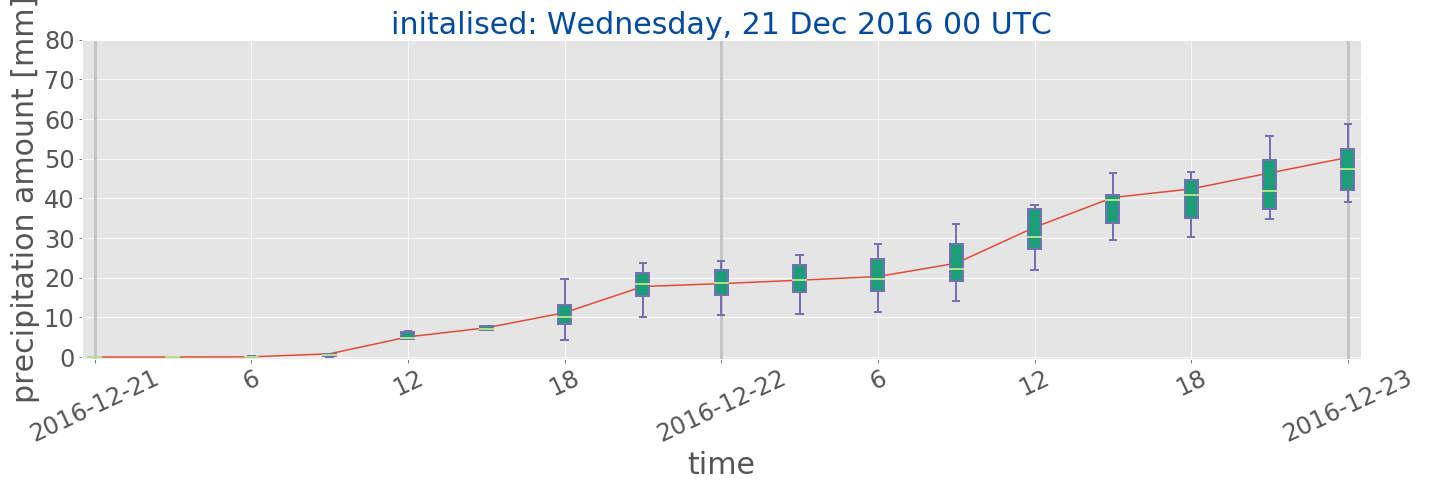
\includegraphics[width=\textwidth]{./fig_boxplot_sfc/20161221_0}
	\caption{Box-whisker-plot of the ten ensemble members of MEPS. Red line indicating the ensemble mean, lower and upper whisker the 25th and 75th percentile, respectively. Light green shows the median of all members and the box represents the middle \SI{50}{\percent} of scores of the precipitation.}\label{fig:boxplt21}
\end{figure}
%%%%%%%%%%%%%%%%%%%%%%%%%%%%%%%%%%%%%%%%%%%%%%%%%%%%%%%%%%%%%%%%%%%%%%%%%%
A box-whisker-plot shows the time evolution of the distribution of the precipitation amount made of ten ensemble members up to \SI{48}{\hour}. Since some ensemble member do not have forecast values every hour provides the box-whisker-plot in \Cref{fig:boxplt21} information every \SI{3}{\hour}. The red line shows the ensemble mean of all ten members. The short light green horizontal line is showing the median, wide vertical box represents the 25th and 75th percentiles, and minimum and maximum values are indicated by the vertical lines.
\\
The box-whisker-plot in \Cref{fig:boxplt21} shows the distribution of the ten ensemble members. In the first \SI{15}{\hour} of the forecast time agree all members well, since the box and whiskers are narrow. With increasing forecast time, increases the uncertainty. After \SI{33}{\hour} is the ensemble mean slightly higher than the median of the data. This shift is associated with the one ensemble member being an outlier.
In general can the surface forecast be trusted, especially up to \SI{24}{\hour} since the values of the ensemble members are well distributed around the mean. Maximum and minimum are not having a too large difference which also shows the small spread between the members.
%%%%%%%%%%%%%%%%%%%%%%%%%%%%%%%%%%%%%%%%%%%%%%%%%%%%%%%%%%%%%%%%%%%%%%%%%%

%%%%%%%%%%%%%%%%%%%%%%%%%%%%%%%%%%%%%%%%%%%%%%%%%%%%%%%%%%%%%%%%%%%%%%%%%%
%%%%%%%%% surface obs %%%%%%%%%%%%%%
\subsection{Saturday, \SI{24}{\dec}}\label{sec:2412:surface}
As discussed early seems the surface precipitation amount on \SI{24}{\dec} not to be influenced by too little precipitation which \cite{muller_arome-metcoop:_2017} showed to be the case for precipitation amount up to \SI{10}{\mm}. 
%%% image surface MEPS boxplot %%%%%%%%%%%%%%%%%%%%%%%%%%%%%%%%%%%%%
\begin{figure}[t]
	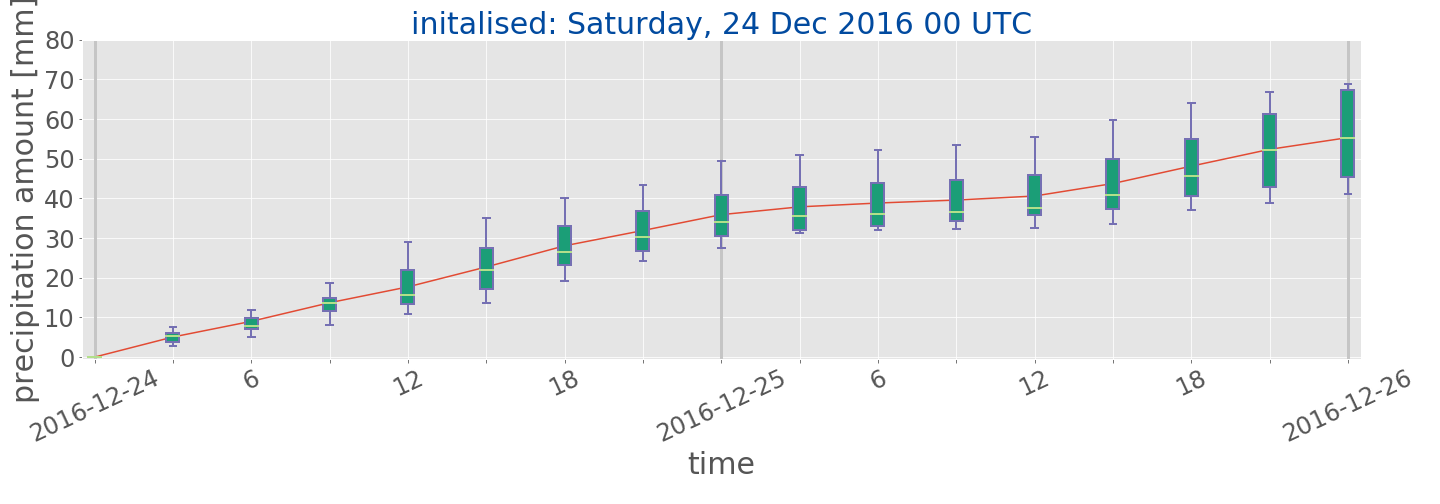
\includegraphics[width=\textwidth]{./fig_boxplot_sfc/20161224_0}
	\caption{Box-whisker-plot of the ten ensemble members of MEPS. Red line indicating the ensemble mean, lower and upper whisker the 25th and 75th percentile, respectively. Light green shows the median of all members and the box represents the middle \SI{50}{\percent} of scores of the precipitation.}\label{fig:boxplt24}
\end{figure}
%%%%%%%%%%%%%%%%%%%%%%%%%%%%%%%%%%%%%%%%%%%%%%%%%%%%%%%%%%%%%%%%%%%%%%%%%%
To understand what might have led to the overestimation of surface precipitation on the \SI{24}{\dec} in \Cref{fig:sfc_acc24}, a box-whisker-plot is presented. Compared to \SI{21}{\dec} shows the box-whisker-plot in \Cref{fig:boxplt24} an uncertainty between the ten ensemble members already after \SI{3}{\hour} forecast time. The spread between the ensemble members (shown by the minimum and maximum whiskers) seems to be wide. Not all ten members agree on the same precipitation amount as they did for example on \SI{21}{\dec}.
\\
The ensemble mean (red line) is always higher than the median and already after \SI{12}{\hour} forecast time is the median closer to the lower 25th percentile. Also, all upper whiskers are taller than the lower ones, which would follow that the ensemble members vary amongst the most positive quartile and that it is very similar for the least positive quartile group.
A comparison with \Cref{fig:sfc_acc24} shows that most of the member lie beneath the ensemble mean (dashed, blue line). On \SI{24}{\dec} the ensemble mean is much lower than the deterministic forecast, which lies closer to the 50th percentile. This is not for all days the case, on most of the days is the ensemble mean either similar or a little less to the deterministic forecast. Since the deterministic forecast, black line in \Cref{fig:sfc_acc24}, is in the upper percentile compared to its perturbed members it follows that for this forecast the deterministic forecast was not the best guess for the surface accumulation and by using the 'wrong' initial state it can have led to larger miscalculations. Therefore, it would be interesting to perform a new deterministic forecast and its associated perturbations to see if a change in choosing another initial state results in a similar measured precipitation amount at the ground.
\\
\\
The uncertainty appearing already after \SI{3}{\hour} can be associated with a too long spin-up time of MEPS. MEPS usually has a spin-up time of about three hours on \SI{25}{\dec} this might have been longer and followed by poorer initial conditions. To represent the surface accumulation well, the model systems needs to be spin-up. The regional model MEPS needs initial and boundary conditions from ECMWF before it can produce forecasts. Since initial conditions such as observations have uncertainties as well as the model has mistrust and needs to approach its own climatology, a model has to stabilize before the simulations can be trusted. The spin-up time varies depending on the quality of the initial and boundary conditions. Apparently, it seems, that the initial and boundary conditions for MEPS were not perfect on \SI{24}{\dec} at \SI{0}{\UTC} since the deterministic and perturbed members seem not to have stabilised yet and show uncertainties in \Cref{fig:boxplt24} from early on.  At this point it might be interesting to re-run the initialisation again with all available observations to see, if that might have an influence on the overestimation observed in \Cref{fig:sfc_acc24}. It might not necessarily be the observations. Since, ECMWF is the boundary condition of MEPS it could also be that the ECMWF forecast did not have reached its stabilised state when MEPS was initiated.
\\
The uncertainty might also have resulted from the fact, that the precipitation around \SI{0}{\UTC} on \SI{24}{\dec} was higher than on the previous days (see, \Cref{fig:TPU}). Where on the previous days the hourly precipitation around \SI{0}{\UTC} was less intense might a big accretion have followed an uncertainty already after \SI{3}{\hour}. MEPS initialised on \SI{24}{\dec} at \SI{0}{\UTC} might have accounted for an additional precipitation at \SI{12}{\UTC} on \SI{24}{\dec} and that led to the strong increase at \SI{13}{\UTC}. This might be a local effect, that a precipitation cell in the model was spatially misplaced or a by a few kilometres or a higher precipitation amount was expected by the model and actually did not occur at Haukeliseter rather at another site close to Haukeliseter, and followed that strong increase after noon. 
\\
It is therefore important as the double fence construction or measurements from the MRR to give models a good initial condition from observations, so that spin-up time can be reduced and model initialisation start at a realistic state.

%%%%%%%%%%%%%%%%%%%%%%%%%%%%%%%%%%%%%%%%%%%%%%%%%%%%%%%%%%%%%%%%%%%%%%%%%%
%%%%%%%%% surface obs %%%%%%%%%%%%%%
\subsection{Sunday, \SI{25}{\dec}}\label{sec:2512:surface}
On \SI{25}{\dec} the surface accumulation for the first \SI{12}{\hour} is \SI{4.3}{\mm} (see \Cref{tab:sfc_acc}). \cite{muller_arome-metcoop:_2017} stated that the deterministic forecast is showing some overestimation if the \SI{12}{\hour} accumulation is less than \SI{10}{\mm}. Even though the surface accretion is smaller than \SI{10}{\mm} might that not correlate with miscalculation on \SI{25}{\dec}. The overestimation started to be pronounced \SI{13}{\hour} after the initialisation in \Cref{fig:sfc_acc25}.
%
%%% image surface MEPS boxplot %%%%%%%%%%%%%%%%%%%%%%%%%%%%%%%%%%%%%
\begin{figure}[t]
	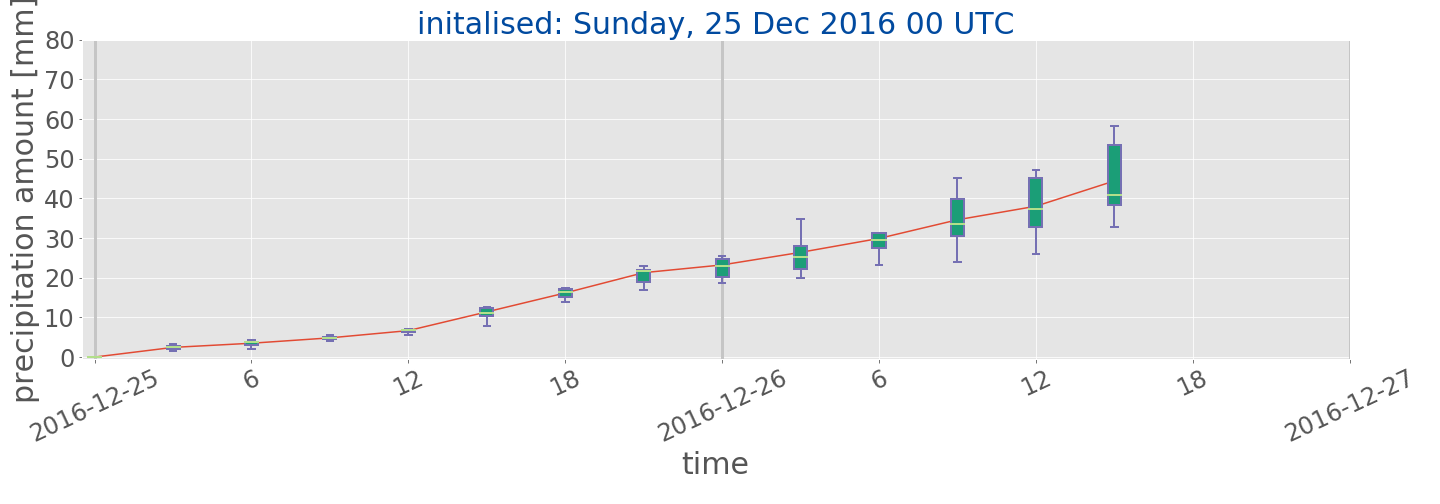
\includegraphics[width=\textwidth]{./fig_boxplot_sfc/20161225_0}
	\caption{Box-whisker-plot of the ten ensemble members of MEPS initialised on \SI{25}{\dec} at \SI{0}{\UTC}. Red line indicating the ensemble mean, lower and upper whisker the 25th and 75th percentile, respectively. Light green shows the median of all members and the box represents the middle \SI{50}{\percent} of scores of the precipitation.}\label{fig:boxplt25}
\end{figure}
%%%%%%%%%%%%%%%%%%%%%%%%%%%%%%%%%%%%%%%%%%%%%%%%%%%%%%%%%%%%%%%%%%%%%%%%%%
%
Compared to \SI{24}{\dec} are the box-whiskers narrower for the first \SI{30}{\hour} on \SI{25}{\dec} in \Cref{fig:boxplt25}. The overestimation started to occur around \SI{13}{\UTC} in \Cref{fig:sfc_acc25}. As \Cref{fig:boxplt25} shows, increases the uncertainty in the forecast after \SI{15}{\UTC}. In general agree median and mean well for the entire period of a \SI{48}{\hour} forecast. After \SI{39}{\hour} prediction time is the mean much higher than the median and closer to the lower 25th percentile in \Cref{fig:boxplt25}. It seems, that all ten ensemble members agree well on the prediction and nevertheless overestimates MEPS the surface accumulation. It shows that the MEPS estimation follows the double fence amount, just not as high. 
\\
In this case it might have been a miscalculation of the occurrence and amount of the precipitation. From the box-whisker-plot (\Cref{fig:boxplt25}) it seems not to be an initialisation problem, since all members agree and the fact that the ensemble mean agrees with the deterministic run. On \SI{25}{\dec} it was expected from the weather maps that a warm front, the warm sector, and a cold front are going to pass. MEPS might have misinterpreted this passages and expected more, probably liquid precipitation associated with the warm front. 
An error associated with the spin-up time of MEPS is not totally excluded. Since the box-whisker-plot shows a good agreement between all members it is not very likely that this was the problem on \SI{25}{\dec}
\\
That the retrieval underestimates the surface precipitation in the afternoon on \SI{25}{\dec} is due to the total negligence  of liquid precipitation if the surface temperature exceeds \SI{2}{\celsius}. Since the optimal estimation retrieval only uses the moist adiabatic lapse rate of \SI{5}{\kelvin\per\km} it might not represent the true state of the atmosphere. Therefore, a use of radiosonde can provide a real structure of the vertical temperature profile which then can help to give real estimations of solid precipitation in the vertical.
After the optimal estimation retrieval is fully developed it will be interesting to study the combination of liquid and snowfall precipitation. 
